 \documentclass[xcolor=dvipsnames,table]{beamer}

\usepackage{latexsym}
\usepackage[utf8]{inputenc}
\usepackage[brazil]{babel}
\usepackage{amssymb}
\usepackage{amsmath}
\usepackage{stmaryrd}
\usepackage{fancybox}
\usepackage{datetime}
\usepackage[T1]{fontenc}
\usepackage{graphicx}
\usepackage{graphics}
\usepackage{url}
\usepackage{algorithmic}
\usepackage{algorithm}
\usepackage{acronym}
\usepackage{array}

\usepackage{enumitem}

\newtheorem{definicao}{Definio}
\newcommand{\tab}{\hspace*{2em}}

\mode<presentation>
{
  \definecolor{colortexto}{RGB}{0,0,0}
 
  \setbeamertemplate{background canvas}[vertical shading][ bottom=white!10,top=white!10]
  \setbeamercolor{normal text}{fg=colortexto} 

  \usetheme{Warsaw}
}

\title{Educação em Computação}  

\author{
  Esdras Lins Bispo Jr. \\ \url{bispojr@ufj.edu.br}
  } 
 \institute{
  Tópicos em Informática e Educação \\Bacharelado em Ciência da Computação}
\date{\textbf{30 de março de 2026} }

\logo{
\includegraphics[width=1.5cm]{images/ufjJataiLogo.png}}

\begin{document}

	\begin{frame}
		\titlepage
	\end{frame}

	\AtBeginSection{
		\begin{frame}{Sumário}%[allowframebreaks]{Sumário}
    		\tableofcontents[currentsection]
    		%\tableofcontents[currentsection, hideothersubsections]
		\end{frame}
	}

	\begin{frame}{Plano de Aula}
		\tableofcontents
		%\tableofcontents[hideallsubsections]
	\end{frame}
	
	\section{Instrução pelos Colegas}

        \begin{frame}{Pesquisa 004}
		\begin{block}{[P004]}
			Como foi a leitura do estudo prévio?
		\end{block}
		\begin{enumerate}[label=(\Alph*)]
			\item Boa leitura
			\item Leitura razoável
			\item Difícil de ler
			\item Não consegui ler
		\end{enumerate}
	\end{frame}

    \section{Pensamento Computacional}
    \begin{frame}{Pensamento Computacional}
        
        O Pensamento Computacional (PC) envolve
        
        \begin{block}{Decomposição}
            Identificar um problema (que pode ser complexo) e quebrá-lo em pedaços menores de mais fácil análise, compreensão e solução.
        \end{block} \pause
        \begin{block}{Reconhecimento de padrões}
            Cada um desses problemas menores pode ser analisado individualmente em profundidade, identificando problemas parecidos que já foram solucionados anteriormente.
        \end{block} 
        
    \end{frame}

    

    \begin{frame}{Pensamento Computacional}
        
        O Pensamento Computacional (PC) envolve
        
        \begin{block}{Abstração}
            Focando apenas nos detalhes que são importantes, enquanto informações irrelevantes são ignoradas.
        \end{block} \pause
        \begin{block}{Algoritmos ou passos}
            Passos ou regras simples podem ser criados para resolver cada um dos subproblemas encontrados.
        \end{block}
        
    \end{frame}

    \begin{frame}{Pensamento Computacional}
        
        \centering
        
        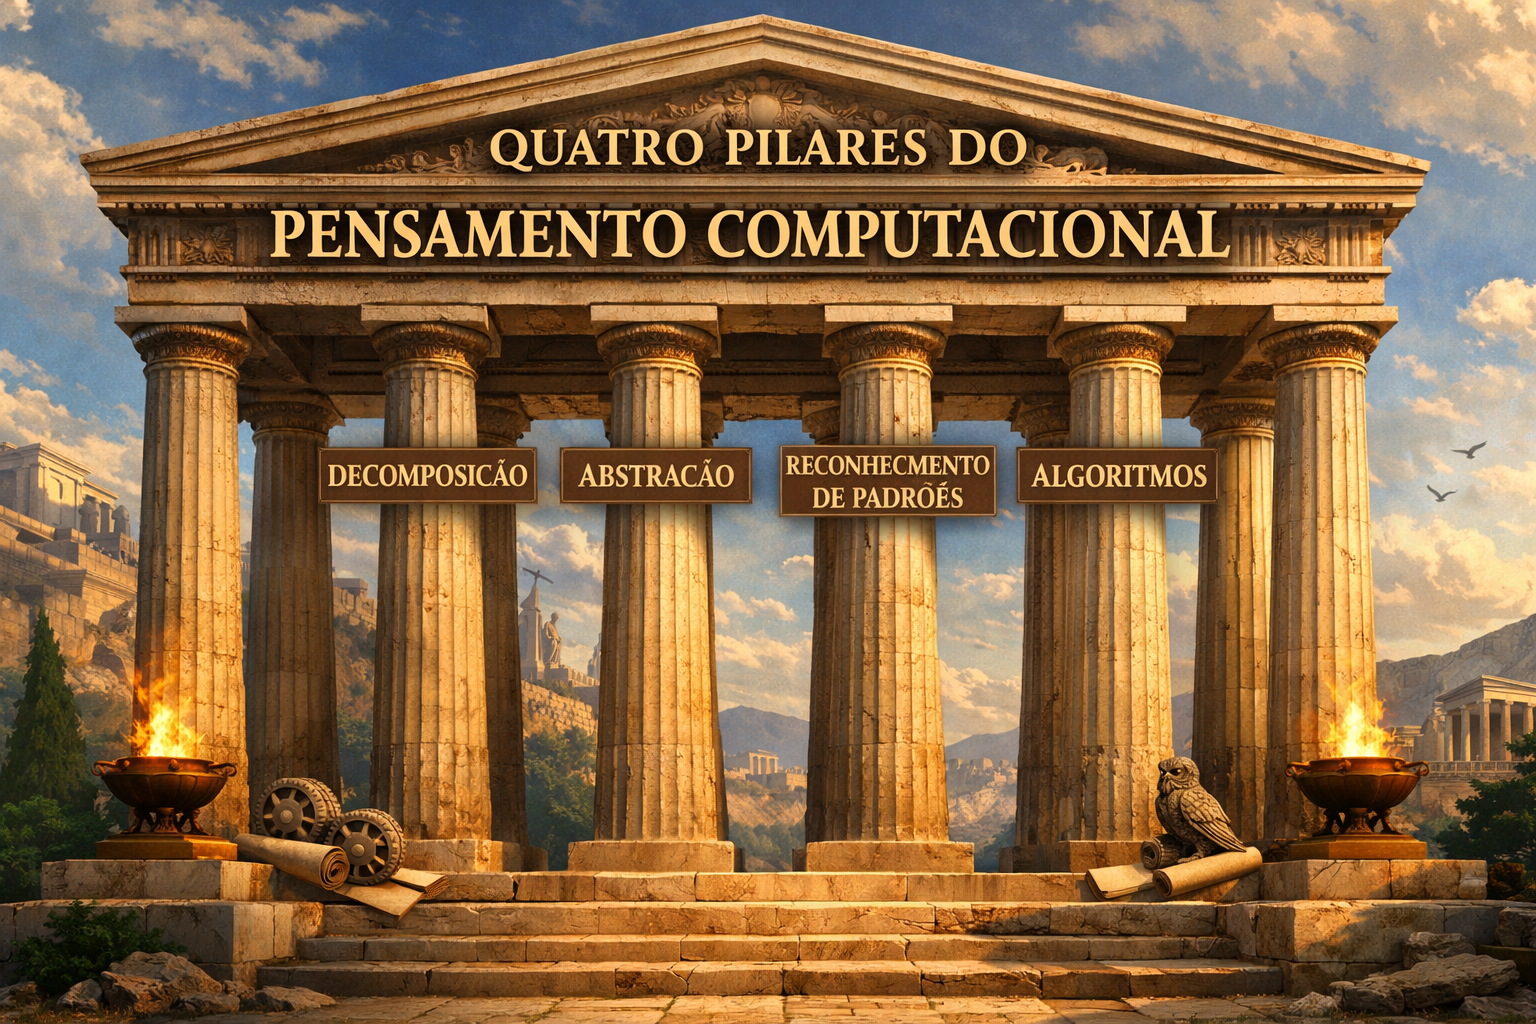
\includegraphics[height=0.8\textheight]{images/pc-pt.png} 
        
    \end{frame}

    \begin{frame}{Questão 012}
		\begin{block}{[Q012]}
		 Um aluno está escrevendo um resumo de um conto infantil. Para isso, ele destaca apenas os personagens principais e os eventos centrais da história, deixando de lado detalhes como a cor das roupas ou o nome da cidade.

        Que pilar do Pensamento Computacional está sendo trabalhado? 
		\end{block}
		\begin{enumerate}[label=(\Alph*)]
			\item Decomposição
                \item Algoritmos
                \item Reconhecimento de padrões
                \item Abstração
		\end{enumerate}
	\end{frame}

	\begin{frame}{Questão 013}
		\begin{block}{[Q013] BNCC Computação}
		 {\bf (EF03CO03)} Aplicar a estratégia de decomposição para resolver problemas complexos, dividindo esse problema em partes menores, resolvendo-as e combinando suas soluções.

        Assinale a alternativa que {\bf melhor representa} o desenvolvimento dessa habilidade em sala de aula: 
		\end{block}
		\begin{enumerate}[label=(\Alph*)]
			\item Um estudante executa um conjunto de instruções previamente definido para resolver um problema.
			\item Um grupo organiza dados em categorias para facilitar sua análise.
			\item Alunos dividem o desenvolvimento de um sistema em módulos independentes e posteriormente integram suas soluções.
			\item Um estudante identifica padrões recorrentes em diferentes problemas para reaproveitar soluções.
		\end{enumerate}
	\end{frame}

        \begin{frame}{Questão 014}
		\begin{block}{[Q014]}
		 Durante uma atividade, uma professora mostrou várias figuras geométricas: quadrados, retângulos e triângulos. Os alunos perceberam que, embora diferentes, todos os quadrados e retângulos tinham ângulos retos e lados paralelos.

Qual pilar do Pensamento Computacional está em evidência nessa situação? 
		\end{block}
		\begin{enumerate}[label=(\Alph*)]
			\item Decomposição
                \item Algoritmos
                \item Reconhecimento de padrões
                \item Abstração
		\end{enumerate}
	\end{frame}

	\begin{frame}[shrink]{Questão 015}
		\begin{block}{[Q015] BNCC Computação}
		 {\bf (EF03CO03)} Criar e simular algoritmos representados em linguagem oral, escrita ou pictográfica, analisando como a precisão da instrução impacta na execução.

        Assinale a alternativa {\bf melhor representa} evidencia essa habilidade: 
		\end{block}
		\begin{enumerate}[label=(\Alph*)]
			\item Um estudante elabora um conjunto de instruções para realizar uma tarefa e as executa corretamente na primeira tentativa.
			\item Um estudante cria instruções para resolver um problema, testa sua execução e as reformula ao perceber falhas causadas por falta de precisão.
			\item Um aluno descreve oralmente os passos de uma atividade e um colega tenta executá-los, mesmo havendo ambiguidades nas instruções.
			\item Um grupo constrói coletivamente um conjunto de passos para resolver um problema, garantindo que todos compreendam a sequência proposta.
		\end{enumerate}
	\end{frame}

    \begin{frame}[shrink]{Questão 016}
		\begin{block}{[Q016]}
		 Um professor propôs a seguinte atividade em sala de aula:
“As crianças devem analisar como funcionam diferentes tipos de bicicletas, identificando partes comuns entre elas, como rodas, pedais e guidão. Depois, deverão criar instruções passo a passo para montar uma bicicleta simples, destacando apenas as informações relevantes e deixando de lado detalhes supérfluos.”

Quais etapas do PC estão sendo aplicadas nessa atividade?

		\end{block}
		\begin{enumerate}[label=(\Alph*)]
			\item Apenas decomposição e algoritmos.
			\item Reconhecimento de padrões, abstração e algoritmos.
			\item Somente abstração.
			\item Decomposição e reconhecimento de padrões. 
		\end{enumerate}
	\end{frame}

    \begin{frame}[shrink]{Questão 017}
	\begin{block}{[Q017] BNCC Computação}
		{\bf (EF01CO01)} Organizar objetos físicos ou digitais considerando diferentes características, explicitando semelhanças e diferenças.

		Assinalea prática pedagógica {\bf mais coerente} com essa habilidade.
	\end{block}
	\begin{enumerate}[label=(\Alph*)]
		\item Agrupar objetos com critérios próprios, justificando semelhanças e diferenças.
		\item Classificar objetos com critérios definidos pelo professor, explicando os agrupamentos.
		\item Organizar objetos seguindo passos predefinidos, garantindo consistência.
		\item Selecionar apenas características relevantes, ignorando as irrelevantes.
	
	\end{enumerate}
\end{frame}

% \section{Próxima Aula}
% \begin{frame}{Próxima Aula}
%     \begin{block}{Leitura Prévia}
%         \begin{itemize}
%             \item WING, J. Pensamento Computacional. Educação e Matemática, n. 162, p. 141-166, 2014. Disponível em: \url{https://em.apm.pt/index.php/em/article/view/2736}.  
%         \end{itemize}
%     \end{block}
%     \begin{block}{Páginas}
%         \begin{itemize}
%         \item Todo o artigo (04 páginas). 
%         \end{itemize}
%     \end{block}
% \end{frame}
	
	\begin{frame}
		\titlepage
	\end{frame}
	
\end{document}